\documentclass[12pt, a4paper]{article}

% Preamble {{{

% Packages {{{

% lang & encoding
\usepackage[utf8]{inputenc}
\usepackage[portuguese]{babel}
\usepackage{csquotes}
\usepackage[T1]{fontenc}
\usepackage{hyphenat}
\usepackage{textcomp} % ordinals: º && ª

% images
\usepackage{graphicx}
\graphicspath{ {./img/} }

% index
\usepackage{imakeidx}
\usepackage[inline]{enumitem}

% tables
\usepackage{tablefootnote}
\usepackage{multirow}
\usepackage{booktabs}

% symbols
\usepackage{gensymb}
\usepackage{amsmath}

% layout and navi
\usepackage{indentfirst} % indent first line of a section
\usepackage[
    hidelinks,
    colorlinks = true,
    linkcolor = blue,
    citecolor = red
]{hyperref}
\usepackage[export]{adjustbox}
\usepackage[
    left=2cm,
    right=2cm,
    top=2cm,
    bottom=2cm
]{geometry}

% }}}

\renewcommand{\baselinestretch}{1.3}
\makeindex

% Keywords
\providecommand{\keywords}[1]
{
    \small
    \textbf{Keywords:} #1
}

% bib
\usepackage[backend=biber, style=ieee,urldate=iso,seconds=true,dateabbrev=false]{biblatex}
\addbibresource{refs.bib}

% fileinfo
\title{
    Resist\^{e}ncia e Energia {\textemdash} T\'ermica
}

\author{
    Marco Maia          {\textemdash}    1210951\\
    R\'{u}ben Ferreira  {\textemdash}    1210954\\
    Jo\~{a}o Teixeira   {\textemdash}    1210957\\
    Jos\'{e} Rente      {\textemdash}    1211155\\
}

% }}}

% start
\begin{document}

% title page {{{
\makeatletter
\begin{titlepage}
	\begin{center}
		\par
		\noindent
		
\includegraphics[
			width=0.3\textwidth,
			valign=M,
			margin=0ex 2ex
		]{isep-logo.png}
		\hfill
		
\includegraphics[
			width=0.3\textwidth,
			valign=M,
			margin=0ex 2ex
		]{dei-logo.png}\\[4ex]
		\par
		{\bfseries  \@title}\\[2ex]
		{\@date}\\[2ex]
		{\@author}
	\end{center}
\end{titlepage}
\makeatother
\thispagestyle{empty}
\newpage

{
    \hypersetup{hidelinks}
    \tableofcontents
    \printindex
    \newpage
}

% }}}

\section{Introdu\c{c}\~ao}\label{sec:intro}

No \^ambito do Projeto Integrador a desenvolver, pretendeu-se elaborar uma estrutura
correspondente a um armaz\'em agr\'{\i}cola dividido em cinco zonas {\textemdash}
A, B, C, D e E {\textemdash}, de forma a poder suportar diferentes temperaturas.

Este relat\'orio tem, portanto, como objetivo detalhar o processo de escolha de materiais
a utilizar na constitui\c{c}\~ao das v\'arias paredes {\textemdash} bem como o telhado
{\textemdash} do armaz\'em e as resist\^encias t\'ermicas respetivamente associadas.

% section Introdução (end)

\section{Seleção de materiais}\label{sec:select}

Perante o problema apresentado, investigar um conjunto de materiais para fazerem parte de uma
estrutura, iniciou-se uma pesquisa em busca das melhores alternativas. Para tal, procurou-se
materiais com um \textbf{baixo valor de condutividade térmica ($k$)}.

\subsection{Paredes Exteriores}\label{sec:pext}

Perante uma situação de diferentes temperaturas nas diversas secções da estrutura, optou-se por manter a consistência
e utilizar os \textbf{mesmos materiais em todas as paredes exteriores}.

No final, obteve-se uma espessura de $32cm$.

\subsubsection{Camada Exterior}\label{sec:pext_ce}

Para a camada exterior das paredes, escolheu-se o \textbf{cimento}. Este material é usado em infraestruturas de todo o mundo
dado, não só às suas \textbf{características térmicas satisfatórias} mas, também, ao seu \textbf{baixo custo}.

Optou-se pela seguinte disposição:

\begin{table}[htpb]
    \begin{center}
        \begin{tabular}{||c c c||}
            \hline
            Material & $k \hspace{1mm} (Wm^{-1}K^{-1})$ & $\Delta x \hspace{1mm} (m)$ \\ [0.5ex]
            \hline\hline
            Cimento  & $0,46$~\cite{concrete}                          & $0,09$                    \\ \hline
        \end{tabular}
    \end{center}
    \caption{Configura\c{c}\~ao da camada exterior}
\end{table}

\subsubsection{Camada Isolante e Estrutural}\label{sec:pext_cie}

Para a camada isolante e estrutural, destacaram-se os seguintes materiais:

\begin{center}
	\begin{itemize}
		\item ICF;
        \item Tijolo refratário, ($k=0,78 \hspace{1mm} Wm^{-1}K^{-1}$)~\cite{brick}.
	\end{itemize}
\end{center}

\begin{figure}[htpb]
	\centering
	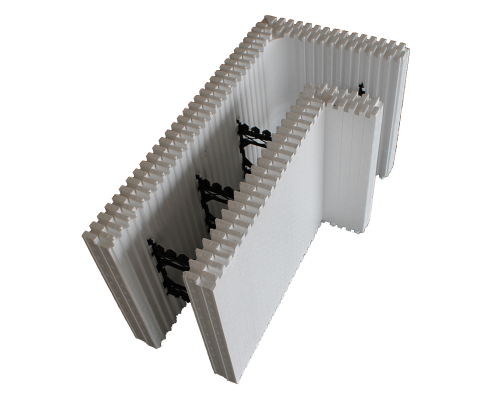
\includegraphics[width=0.3\textwidth]{icf-exemplo.png}

	\caption{Sistema ICF, ainda por preencher com betão armado}\label{fig:icf1}
\end{figure}

Entre ambos, foi decidido utilizar o ICF.\@ O ICF é uma sistema de construção distinguido pelo seu elevado
\textbf{isolamento térmico} e acústico, baixo custo de manutenção e fácil aplicação. Este sistema é constituído por
\textbf{dois blocos isolantes verticais} de \textbf{poliestireno expandido} que, após a sua respetiva montagem,
são preenchidos por \textbf{betão armado}.


Tendo sido desenvolvidos há pouco mais de 30 anos, estes sistemas têm sido utilizados um pouco por todo o mundo,
com especial ênfase nos EUA e no Canadá, dadas as suas ótimas capacidades \textbf{térmicas} e acústicas

Apesar de, na figura~\ref{fig:icf1}, estar representado um reforço com barras de metal, essas serão
ignoradas neste trabalho experimental.

Optou-se pela seguinte disposição:

\begin{table}[htpb]
    \begin{center}
        \begin{tabular}{||c c c||}
            \hline
            Material               & $k \hspace{1mm} (Wm^{-1}K^{-1})$ & $\Delta x \hspace{1mm} (m)$ \\ [0.5ex]
            \hline\hline
            Poliestireno Expandido & $0,037$~\cite{poliestireno_k}          & $0,02$                      \\
            \hline
            Betão Armado           & $2$~\cite{betao_armado}                  & $0,18$                      \\
            \hline
            Poliestireno Expandido & $0,037$                          & $0,02$                      \\
            \hline
        \end{tabular}
    \end{center}
    \caption{Configura\c{c}\~ao da camada isolante e estrutural}
\end{table}

\subsubsection{Camada Interior}\label{pext_ci}

Para a camada interior, destacaram-se os seguintes materiais:

\begin{itemize}
    \item Gesso, ($k=0,25 \hspace{1mm} Wm^{-1}K^{-1}$)
    \item Estuque, ($k=0,4 \hspace{1mm} Wm^{-1}K^{-1}$)
\end{itemize}

Pelas claras diferenças nos valores de condutividade térmica, escolheu-se o \textbf{gesso} para o revestimento interior
das paredes exteriores.

\pagebreak
Optou-se pela seguinte disposição:

\begin{table}[htpb]
    \begin{center}
        \begin{tabular}{||c c c||}
            \hline
            Material & $k \hspace{1mm} (Wm^{-1}K^{-1})$ & $\Delta x \hspace{1mm} (m)$ \\ [0.5ex]
            \hline\hline
            Gesso    & $0,25$~\cite{gesso_k}                          & $0,01$                      \\
            \hline
        \end{tabular}
    \end{center}
    \caption{Configura\c{c}\~ao da camada interior}
\end{table}

\subsection{Paredes Interiores}\label{sub:paredes_int}

Relativamente \`as paredes interiores, estas foram divididas em duas categorias {\textemdash}
\textbf{Estruturais} e \textbf{N\~ao Estruturais} {\textemdash}, sendo que o facto de ser
uma parede estrutural teve influ\^encia na escolha do materiais e da sua respetiva espessura.

\subsubsection{Camada Exterior e Interior}\label{ssub:paredes_int_ext}

Relativamente \`as paredes interiores, optou-se por utilizar o \textbf{gesso} como material
para a camada exterior de ambos os lados das paredes, pois trata-se de um composto que
enfortece~\cite{gesso_vantagens} as paredes e, visto que estas s\~ao as camadas
vis\'{\i}veis \`aqueles que circulam pelo armaz\'em, conv\'em conferir um certo
valor est\'etico \`as paredes. Para al\'em disso, o gesso \'e um material relativamente barato
e possui uma condutividade t\'ermica apreci\'avel ($ k = 0.25 \hspace{1mm} Wm^{-1}K^{-1} $)
para o contexto~\cite{gesso_k}.

\begin{table}[htpb]
    \begin{center}
        \begin{tabular}{c c c}
            \toprule{}
            Material & $ k \hspace{1mm} (Wm^{-1}K^{-1}$) & $ \Delta x \hspace{1mm} (m)$ \\
            \midrule{}
            Gesso & $0.25$ & $0.01$ \\
            \bottomrule{}
        \end{tabular}
    \end{center}
    \caption{Dados da componente exterior}\label{tab:parede_int_ext}
\end{table}

% subsubsection Camada Exterior (end)

\subsubsection{Camada Isolante e Estrutural}\label{ssub:paredes_int_isolante}

Para as paredes estruturais, o material escolhido foi o ICF, pelas mesmas raz\~oes referidas
acima na sec\c{c}\~ao~\ref{sec:pext_cie}.
J\'a para as n\~ao estruturais, como estas n\~ao necessitam suportar bastante o edif\'{\i}cio,
foi decidido utilizar um composto de \textbf{Poliestireno extrudido} e de
\textbf{Madeira Pinus}. \'E no entanto, relevante mencionar que o poliestireno possui um
excelente desempenho t\'ermico ($ k = 0.033 \hspace{1mm} Wm^{-1}K^{-1} $)~\cite{poliestireno_k}
e \'e de uma elevada rapidez de instala\c{c}\~ao~\cite{poliestireno}.

\begin{table}[htpb]
    \begin{center}
        \begin{tabular}{c c c}
            \toprule{}
            Material & $ k \hspace{1mm} (Wm^{-1}K^{-1}$) & $ \Delta x \hspace{1mm} (m)$ \\
            \midrule{}
            Poliestireno extrudido & $0.033$ & $0.02$ (estrutural) \\
            \midrule{}
            Bet\~ao armado & $2$ & $0.18$ \\
            \midrule{}
            Poliestireno extrudido & $0.033$ & $0.08$ (n\~ao estrutural) \\
            \midrule{}
            Madeira Pinus & $0.12$ & $0.1$ \\
            \bottomrule{}
        \end{tabular}
    \end{center}
    \caption{Dados da componente isolante}\label{tab:parede_int_iso}
\end{table}


% subsubsection Camada Isolante e Estrutural (end)

\pagebreak
\subsection{Telhado}\label{sub:Telhado}

Para o telhado, optou-se por um modelo de duas águas. Para a \textbf{estrutura exterior}, o que fez mais sentido foi
uma cobertura de \textbf{cimento}, sobreposto por uma camada de \textbf{telha}. O cimento, pelas mesmas razões referidas no tópico~\ref{sec:pext_ce}, foi a melhor decisão, dado aos seus baixos valores de condutividade térmica de $k=0,46 \hspace{1mm} Wm^{-1}K^{-1}$.

Já o \textbf{material isolante} escolhido, difere do material isolante das paredes exteriores. Optou-se
por \textbf{espuma de poliuretano} que, permite obter um isolamento térmico que satisfaz as necessidades
do caso de estudo. Este material apresenta um valor de condutividade térmica de
$k=0,028 \hspace{1mm} Wm^{-1}K^{-1}$~\cite{poliuretano} e, é muito popular nas indústrias que dependem de \textbf{espaços
	com temperaturas controladas}.

\begin{figure}[htpb]
	\centering
	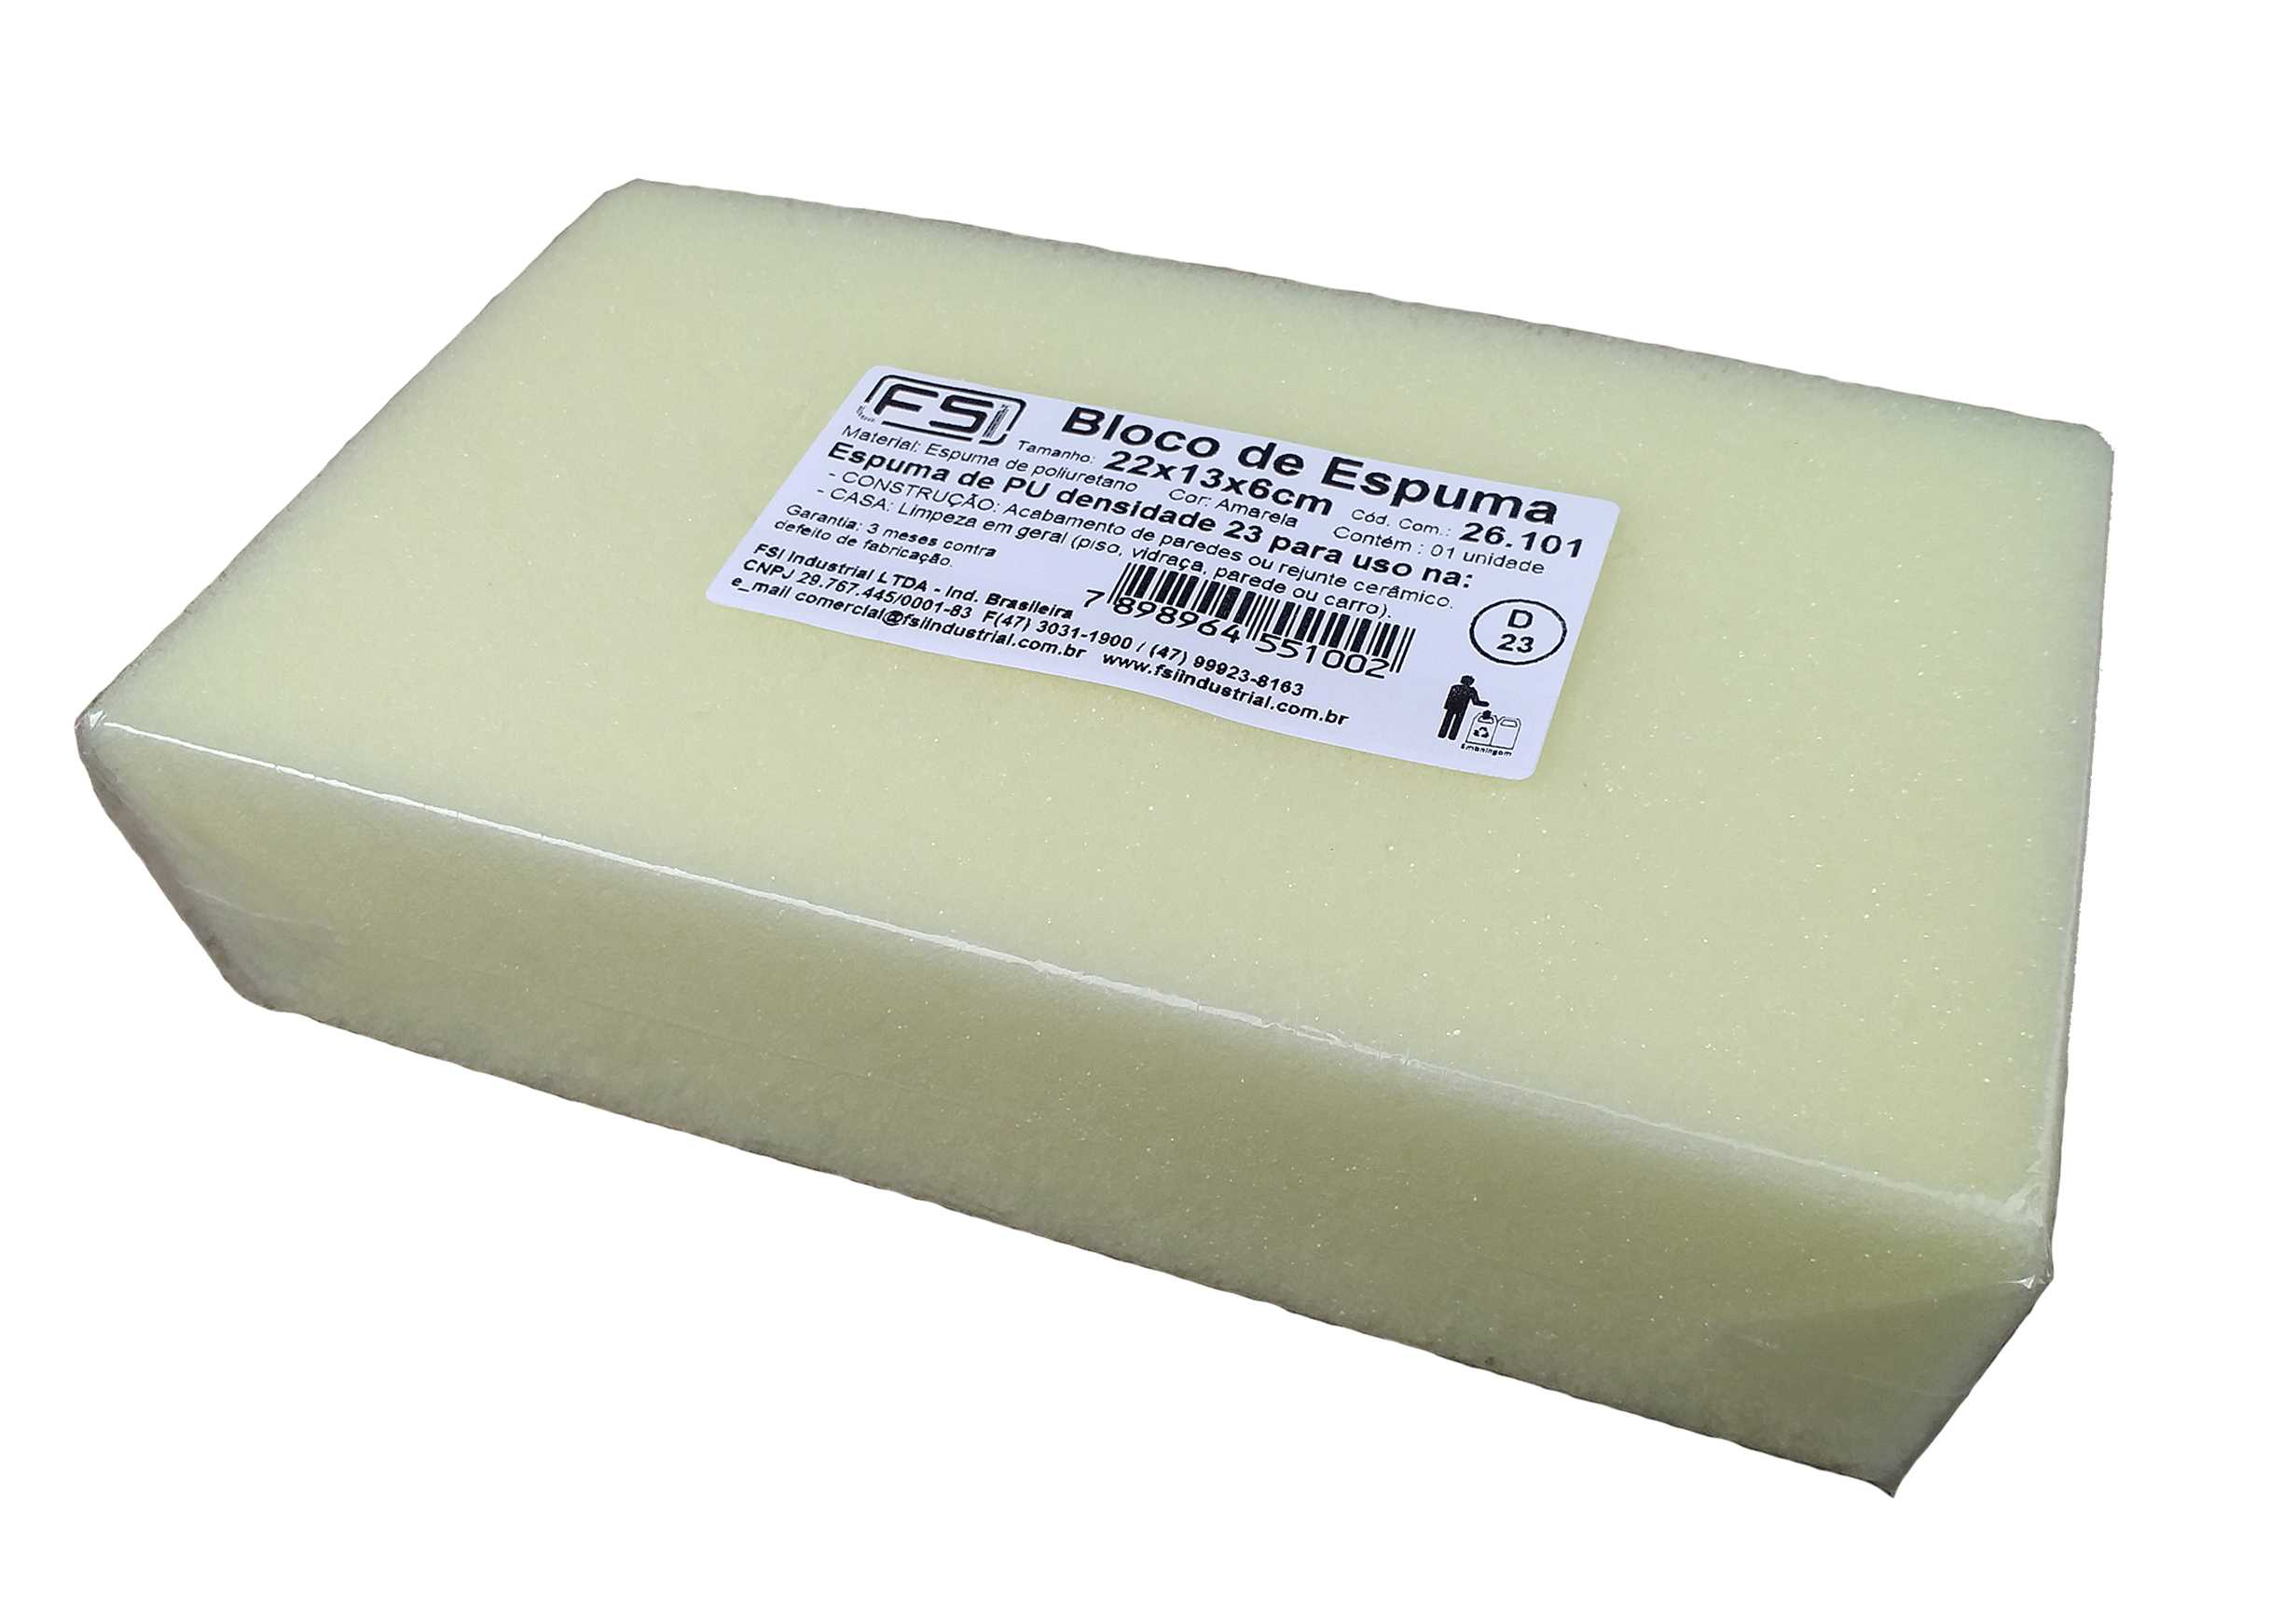
\includegraphics[width=0.3\textwidth]{espuma_poliuretano.jpg}
	\caption{Espuma de poliuretano}\label{fig:poliuretano}
\end{figure}

Por fim, e, à semelhança das paredes exteriores, decidiu-se aplicar uma camada de \textbf{gesso}, como
\textbf{revestimento interior do telhado}.

Optou-se pela seguinte disposição:

\begin{center}
	\begin{tabular}{||c c c c||}
		\hline
		Estrutura & Material              & $k \hspace{1mm} (Wm^{-1}K^{-1})$ & $\Delta x \hspace{1mm} (m)$ \\ [0.5ex]
		\hline\hline
		Exterior  & Telha                 & $1,2$                            & $0,06$                      \\
		\hline
		Cobertura & Cimento               & $0,46$                           & $0,04$                      \\
		\hline
		Isolante  & Espuma de Poliuretano & $0,028$                          & $0,17$                      \\
		\hline
		Interior  & Gesso                 & $0,25$                           & $0,03$                      \\
		\hline
	\end{tabular}
\end{center}

% subsection Telhado (end)


\subsection{Portas}\label{sub:Portas}

De acordo com o enunciado providenciado pelo cliente, o armaz\'em possuir\i{\i}a
tr\^es tipos de portas

\begin{enumerate}
    \item Porta de subir {\textemdash} Zona A
    \item Porta de duas folhas (dupla) {\textemdash} Zona B
    \item Porta simples {\textemdash} Restantes zonas
\end{enumerate}

Na escolha dos materiais n\~ao se achou necessidade de distinguir os materiais a
usar na constitui\c{c}ao da porta dupla e das simples e, portanto, decidiu-se
utilizar a \textbf{Madeira Pinus}.

J\'a para a porta de vidro, decidiu-se utilizar uma configura\c{c}\~ao com fibra de vidro.

\begin{table}[htpb]
    \begin{center}
        \begin{tabular}{c c c}
            \toprule{}
            Material & $ k \hspace{1mm} (Wm^{-1}K^{-1}$) & $ \Delta x \hspace{1mm} (m)$ \\
            \midrule{}
            Madeira Pinus & $0.12$~\cite{pine_wood} & $0.1$ \\
            \midrule{}
            Fibra de Vidro & $0.04$~\cite{glass_fiber} & $0.1$ \\
            \bottomrule{}
        \end{tabular}
    \end{center}
    \caption{Dados da constitui\c{c}\~ao das portas}\label{tab:portas}
\end{table}

% subsection Portas (end)


\subsection{Janelas}\label{sub:Janelas}

Por fim, foram idealizadas duas janelas que satisfazem as necessidades térmicas do espaço.
Para tal, optou-se por uma construção de \textbf{duas folhas}, com uma \textbf{estrutura de alumínio} e
vidro duplo.

\begin{table}[htpb]
    \begin{center}
        \begin{tabular}{||c c c c||}
            \hline
            Estrutura & Material & $k \hspace{1mm} (Wm^{-1}K^{-1})$ & $\Delta x \hspace{1mm} (m)$ \\ [0.5ex]
            \hline\hline
            Perfil    & Alumínio & $237$                            & $0,053$                     \\
            \hline
            Vidro     & Vidro    & $0,79$                           & $0,004$                     \\
            \hline
            Ar        & Ar       & $0,025$                          & $0,023$                     \\
            \hline
            Vidro     & Vidro    & $0,79$                           & $0,004$                     \\
            \hline
        \end{tabular}
    \end{center}
    \caption{Configura\c{c}\~ao das janelas}
\end{table}

% subsection Janelas (end)


%section Selecao de materiais (end)



\section{Estrutura}\label{sec:Estrutura}

\subsection{Croqui}\label{sub:croqui}

Ap\'os a sele\c{c}\~ao de todos os materiais e a decis\~ao das suas respetivas larguras,
obtivemos a seguinte estrutura para responder ao problema apresentado pelo cliente.

\begin{figure}[htpb]
    \begin{center}
        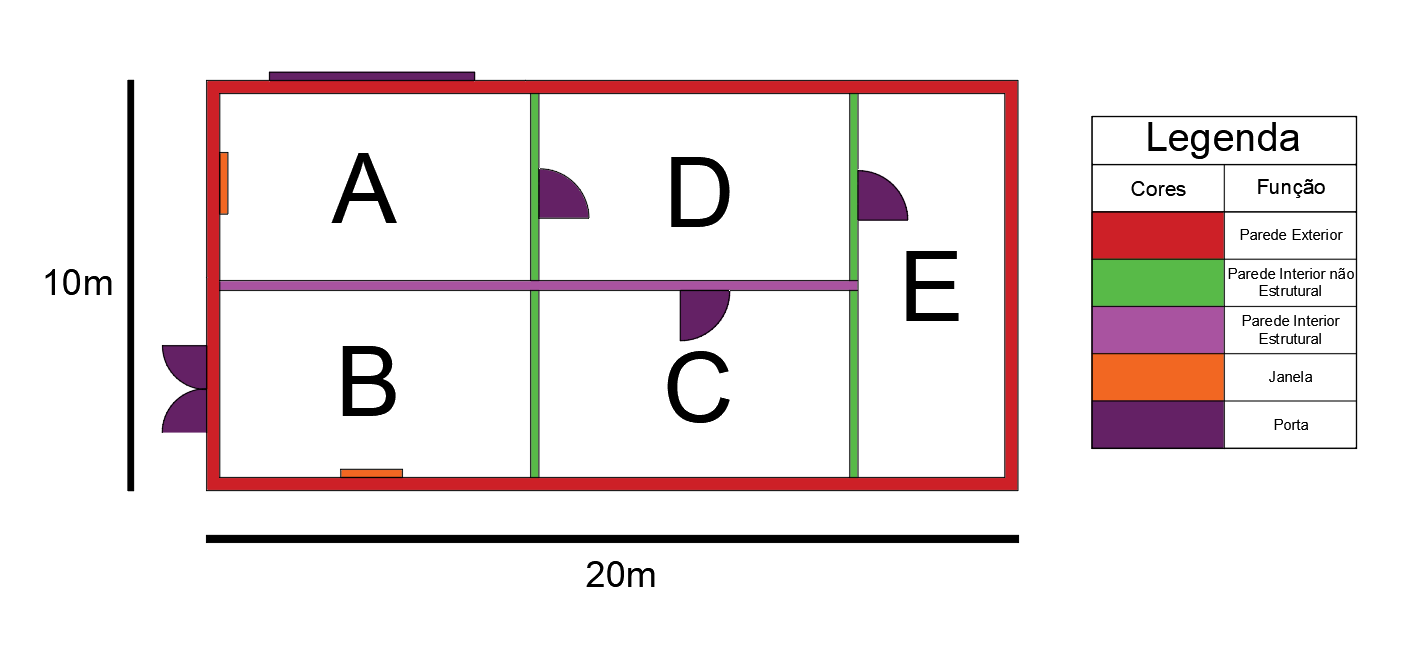
\includegraphics[width=0.95\textwidth]{img/sketch4.png}
    \end{center}
    \caption{Croqui da estrutura concebida}\label{fig:croqui}
\end{figure}

% subsection Croqui (end)


\subsection{Resist\^encia T\'ermica nas Sec\c{c}\~oes}\label{sub:Resistencia Termica nas Seccoes}

\subsubsection{Zona A}\label{ssub:zonaa}

Tendo em conta os materiais apresentados na secção e, o croqui da estrutura, \textbf{a zona A}, para funcionar
à temperatura de $ 15^\circ C $ possui as seguintes características:

\pagebreak
\begin{table}[htpb]
	\begin{center}
		\begin{tabular}{c c c c c}
			\toprule{}
			Secção                     & Material               & $ k \hspace{1mm} (Wm^{-1}K^{-1}$) & $ \Delta x \hspace{1mm} (m)$ & Área $(m^2) $ \\
				\midrule{}

				% Exterior
			\multirow{5}{*}{}          & Cimento                & $0.46$                            & $0.09$                       & $48,5$          \\
				\cline{2-5}
			Parede                     & Poliestireno Expandido & $0.037$                           & $0.02$                       & $48,5$          \\
				\cline{2-5}
			Exterior                   & Betão Armado           & $2$                               & $0.18$                       & $48,5$          \\
				\cline{2-5}
			($\times 2$)               & Poliestireno Expandido & $0.037$                           & $0.02$                       & $48,5$          \\
				\cline{2-5}
			                           & Gesso                  & $0.25$                            & $0.01$                       & $48,5$          \\
				\midrule{}

				% Interior não estrutural
			Parede \multirow{4}{*}{}   & Gesso                  & $0.25$                            & $0.01$                       & $40$          \\
				\cline{2-5}
			Interior                   & Poliestireno Extrudido & $0.033$                           & $0.08$                       & $40$          \\
				\cline{2-5}
			Não Estrutural             & Madeira Pinus          & $0.12$                            & $0.1$                        & $40$          \\
				\cline{2-5}
			($\times 1$)               & Gesso                  & $0.25$                            & $0.01$                       & $40$          \\
				\midrule{}

				% Interior estrutural
			\multirow{5}{*}{}          & Gesso                  & $0.25$                            & $0.01$                       & $37$          \\
				\cline{2-5}
			Parede                     & Poliestireno Extrudido & $0.033$                           & $0.02$                       & $37$          \\
				\cline{2-5}
			Interior                   & Betão Armado           & $2$                               & $0.18$                       & $37$          \\
				\cline{2-5}
			Estrutural ($\times 1$)    & Poliestireno Extrudido & $0.033$                           & $0.02$                       & $37$          \\
				\cline{2-5}
			                           & Gesso                  & $0.25$                            & $0.01$                       & $37$          \\
				\midrule{}

			\multirow{5}{*}{}		   & Alumínio 				& $237$                            	& $0,053$                      & $0,66$		   \\
				\cline{2-5}
			Janela    				   & Vidro    				& $0,79$                           	& $0,004$                      & $1,34$		   \\
				\cline{2-5}
			($\times 1$)			   & Ar       				& $0,025$                          	& $0,023$                      & $1,34$		   \\
				\cline{2-5}
									   & Vidro    				& $0,79$                           	& $0,004$                      & $1,34$		   \\
				\midrule{}
				% Porta
			Porta de Subir ($\times 1$) & Fibra de vidro        & $0.04$                            & $0.1$                        & $15$           \\
			\bottomrule{}
		\end{tabular}
	\end{center}
	\caption{Composição da zona A}\label{tab:zona_a}
\end{table}

Com base na tabela~\ref*{tab:zona_a}, o cálculo das resistências para esta sucede-se da seguinte forma:

\paragraph{Janela:}\label{par:zona_a_janela}Os vidros e o ar estão associados em série:

\begin{equation}
	R_{janelas} = \dfrac{1}{\dfrac{1}{R_{aluminio}} + \dfrac{1}{2 \times R_{vidro} + R_{ar}}}
	\label{eq:zona_a_janelas}
\end{equation}

\begin{equation}
	\Leftrightarrow
	R_{janelas} =
	\dfrac{1}{
		\dfrac{1}{
			\dfrac{0.053}{237 \times 0.66}
		}+
		\dfrac{1}{
			2 \times \dfrac{0.004}{0.79 \times 1.34} +
			\dfrac{0.023}{0.025 \times 1.34}
		}
	}
		= 3.40 \times 10^{-4} \hspace{1mm} KW^{-1}
	\label{eq:zona_a_janelas2}
\end{equation}

% paragraph Janelas (end)

\pagebreak
\paragraph{Parede Exterior com Porta da Subir e Janela:}\label{par:zona_a_ext}Camadas associadas em série:

\begin{equation}
    \dfrac{1}{R}=
		\dfrac{1}{
			R_{cimento} + 2 \times R_{poliestireno} + R_{bet\tilde{a}o} + R_{gesso}
		}
		+
		\dfrac{1}{
			R_{porta\_subir}
		}
		+
		\dfrac{1}{
			R_{janela}
		}
    \label{eq:zona_a_ext_1}
\end{equation}

\begin{equation}
    \Leftrightarrow \dfrac{1}{R}=
		\dfrac{1}{
			\dfrac{0.09}{0.460 \times 48.5} +
			2 \times \dfrac{0.02}{0.037 \times 48.5} +
			\dfrac{0.18}{2 \times 48.5} +
			\dfrac{0.01}{0.25 \times 48.5}
        }
		+
		\dfrac{1}{
        	\dfrac{0.1}{0.04 \times 15}
		}
		+
		\dfrac{1}{
        	3.40 \times 10^{-4}
		}
    \label{eq:zona_a_ext_2}
\end{equation}

\begin{equation}
	\Leftrightarrow R_{parede\_ext + porta + janela} = 3.35 \times 10^{-4} \hspace{1mm} KW^{-1}
	\label{eq:zona_a_ext_3}
\end{equation}

\paragraph{Parede Interior N\~ao Estrutural com porta:}\label{par:zona_a_int_n_est}Paralelo entre a parede e a porta.

\begin{equation}
    \dfrac{1}{R} =
			\dfrac{1}{
            2 \times R_{gesso} + R_{poliestireno\_extrudido} + R_{madeira\_pinus}
			}
			+
			\dfrac{1}{
				R_{porta}
			}
    \label{eq:zona_a_int_n_est_1}
\end{equation}

\begin{equation}
    \Leftrightarrow \dfrac{1}{R} =
			\dfrac{1}{
            2 \times \dfrac{0.01}{0.25 \times 40} +
            \dfrac{0.08}{0.033 \times 40} +
            \dfrac{0.1}{0.12 \times 40}
        	}
			+
			\dfrac{1}{
            \dfrac{0.1}{0.12 \times 3}
			}
    \label{eq:zona_a_int_n_est_2}
\end{equation}

\begin{equation}
    \Leftrightarrow \dfrac{1}{R_{parede\_n\tilde{a}o\_estrut + porta}} =
	\dfrac{1}{
        8.34 \times 10^{-2}
	} +
	\dfrac{1}{
    	2.78 \times 10^{-1}
	}
	= 6.42 \times 10^{-2} \hspace{1mm} KW^{-1}
    \label{eq:zona_a_int_n_est_3}
\end{equation}

\paragraph{Parede Interior Estrutural:}\label{par:zona_a_int_est}

\begin{equation}
	R= 2 \times R_{gesso} + 2 \times R_{poliestireno} + R_{bet\tilde{a}o}
	\label{eq:zona_a_int_est_1}
\end{equation}

\begin{equation}
	\Leftrightarrow R_{parede\_estrut} =
		2 \times \dfrac{0.01}{0.25 \times 37} +
		2 \times \dfrac{0.02}{0.033 \times 37} +
		\dfrac{0.18}{2 \times 37}
		= 3.74 \times 10^{-2} \hspace{1mm} KW^{-1}
	\label{eq:zona_a_int_est_2}
\end{equation}


\paragraph{Total:}\label{par:zona_a_total} Tendo em conta que os componentes est\~ao
associados em série e considerando os resultados das
equa\c{c}\~oes~\ref*{eq:zona_a_ext_3},~\ref*{eq:zona_a_int_n_est_3} e~\ref*{eq:zona_a_int_est_2}

\begin{equation}
	R_{total} =
	\dfrac{1}{
		\dfrac{1}{
		3.35 \times 10^{-4}
		} +
		\dfrac{1}{
		6.42 \times 10^{-2}
		} +
		\dfrac{1}{
		3.74 \times 10^{-2}
		}
	}
	= 3.31 \times 10^{-4} \hspace{1mm} KW^{-1}
	\label{eq:zona_a_total}
\end{equation}

\pagebreak
\subsubsection{Zona B}\label{ssub:zonab}

Tendo em conta os materiais apresentados na secção e, o croqui da estrutura, \textbf{a zona B}, para funcionar
à temperatura de $ 20^\circ C $ possui as seguintes características:

\begin{table}[htpb]
	\begin{center}
		\begin{tabular}{c c c c c}
			\toprule{}
			Secção                     & Material               & $ k \hspace{1mm} (Wm^{-1}K^{-1}$) & $ \Delta x \hspace{1mm} (m)$ & Área $(m^2) $ \\
				\midrule{}

				% Exterior
			\multirow{5}{*}{}          & Cimento                & $0.46$                            & $0.09$                       & $57.5$          \\
				\cline{2-5}
			Parede                     & Poliestireno Expandido & $0.037$                           & $0.02$                       & $57.5$          \\
				\cline{2-5}
			Exterior                   & Betão Armado           & $2$                               & $0.18$                       & $57.5$          \\
				\cline{2-5}
			($\times 2$)               & Poliestireno Expandido & $0.037$                           & $0.02$                       & $57.5$          \\
				\cline{2-5}
			                           & Gesso                  & $0.25$                            & $0.01$                       & $57.5$          \\
				\midrule{}

				% Interior não estrutural
			Parede \multirow{4}{*}{}   & Gesso                  & $0.25$                            & $0.01$                       & $25$          \\
				\cline{2-5}
			Interior                   & Poliestireno Extrudido & $0.033$                           & $0.08$                       & $25$          \\
				\cline{2-5}
			Não Estrutural             & Madeira Pinus          & $0.12$                            & $0.1$                        & $25$          \\
				\cline{2-5}
			($\times 1$)               & Gesso                  & $0.25$                            & $0.01$                       & $25$          \\
				\midrule{}

				% Interior estrutural
			\multirow{5}{*}{}          & Gesso                  & $0.25$                            & $0.01$                       & $40$          \\
				\cline{2-5}
			Parede                     & Poliestireno Extrudido & $0.033$                           & $0.02$                       & $40$          \\
				\cline{2-5}
			Interior                   & Betão Armado           & $2$                               & $0.18$                       & $40$          \\
				\cline{2-5}
			Estrutural ($\times 1$)    & Poliestireno Extrudido & $0.033$                           & $0.02$                       & $40$          \\
				\cline{2-5}
			                           & Gesso                  & $0.25$                            & $0.01$                       & $40$          \\
				\midrule{}

			\multirow{5}{*}{}		   & Alumínio 				& $237$                            	& $0,053$                      & $0,66$		   \\
				\cline{2-5}
			Janela    				   & Vidro    				& $0,79$                           	& $0,004$                      & $1,34$		   \\
				\cline{2-5}
			($\times 1$)			   & Ar       				& $0,025$                          	& $0,023$                      & $1,34$		   \\
				\cline{2-5}
									   & Vidro    				& $0,79$                           	& $0,004$                      & $1,34$		   \\
				\midrule{}
				% Porta
			Porta dupla ($\times 1$)   & Madeira Pinus          & $0.12$                            & $0.1$                        & $6$           \\
			\bottomrule{}
		\end{tabular}
	\end{center}
	\caption{Composição da zona B}\label{tab:zona_b}
\end{table}

Com base na tabela~\ref*{tab:zona_b}, o cálculo das resistências para esta secção sucede-se da seguinte forma:

\paragraph{Janela:}\label{par:zona_b_janela}Os vidros e o ar estão associados em série:

\begin{equation}
	\dfrac{1}{R} = \dfrac{1}{R_{aluminio}} + \dfrac{1}{2 \times R_{vidro} + R_{ar}}
	\label{eq:zona_b_janelas}
\end{equation}

\begin{equation}
	\Leftrightarrow
	\dfrac{1}{R_{janelas}} =
		\dfrac{1}{
			\dfrac{0.053}{237 \times 0.66}
		}+
		\dfrac{1}{
			2 \times \dfrac{0.004}{0.79 \times 1.34} +
			\dfrac{0.023}{0.025 \times 1.34}
		}
		= 3.40 \times 10^{-4} \hspace{1mm} KW^{-1}
	\label{eq:zona_b_janelas2}
\end{equation}

% paragraph Janelas (end)

\paragraph{Parede Exterior com Porta Dupla e Janela:}\label{par:zona_b_ext}Camadas associadas em série:

\begin{equation}
    \dfrac{1}{R} =
			\dfrac{1}{
			R_{cimento} + 2 \times R_{poliestireno} + R_{bet\tilde{a}o} + R_{gesso}
			}
			+
			\dfrac{1}{
				R_{porta\_dupla}
			}
			+
			\dfrac{1}{
				R_{janela}
			}
    \label{eq:zona_b_ext_1}
\end{equation}

\begin{equation}
    \Leftrightarrow \dfrac{1}{R} =
			\dfrac{1}{
				\dfrac{0.09}{0.46 \times 57.5} +
				2 \times \dfrac{0.02}{0.037 \times 57.5} +
				\dfrac{0.18}{2 \times 57.5} +
				\dfrac{0.01}{0.25 \times 57.5}
        	}
			+
			\dfrac{1}{
            	\dfrac{0.1}{0.12 \times 6}
			}
			+
			\dfrac{1}{
            	3.40 \times 10^{-4}
			}
    \label{eq:zona_b_ext_2}
\end{equation}

\begin{equation}
	\Leftrightarrow R_{parede\_ext + porta\_dupla + janela} = 3.34 \times 10^{-4} \hspace{1mm} KW^{-1}
	\label{eq:zona_b_ext_3}
\end{equation}

\paragraph{Parede Interior N\~ao Estrutural:}\label{par:zona_b_int_n_est}

\begin{equation}
	R_{parede\_n\tilde{a}o\_estrut} = 2 \times R_{gesso} + R_{poliestireno\_extrudido} + R_{madeira\_pinus}
	\label{eq:zona_b_int_n_est_1}
\end{equation}

\begin{equation}
	\Leftrightarrow R_{parede\_n\tilde{a}o\_estrut} =
	2 \times \dfrac{0.01}{0.25 \times 25} +
	\dfrac{0.08}{0.033 \times 25} +
	\dfrac{0.1}{0.12 \times 25} = 1.34 \times 10^{-1} \hspace{1mm} KW^{-1}
	\label{eq:zona_b_int_n_est_2}
\end{equation}

\paragraph{Parede Interior Estrutural:}\label{par:zona_b_int_est}

\begin{equation}
	R_{parede\_estrut} = 2 \times R_{gesso} + 2 \times R_{poliestireno} + R_{bet\tilde{a}o}
	\label{eq:zona_b_int_est_1}
\end{equation}

\begin{equation}
	\Leftrightarrow R_{parede\_estrut} =
		2 \times \dfrac{0.01}{0.25 \times 40} +
		2 \times \dfrac{0.02}{0.033 \times 40} +
		\dfrac{0.18}{2 \times 40}
		= 3.46 \times 10^{-2} \hspace{1mm} KW^{-1}
	\label{eq:zona_b_int_est_2}
\end{equation}


\paragraph{Total:}\label{par:zona_b_total} Tendo em conta que os componentes est\~ao
associados em série e considerando os resultados das
equa\c{c}\~oes~\ref*{eq:zona_b_ext_3},~\ref*{eq:zona_b_int_n_est_2} e~\ref*{eq:zona_b_int_est_2}

\begin{equation}
	R_{total} =
	\dfrac{1}{
		\dfrac{1}{
		3.34 \times 10^{-4}
		} +
		\dfrac{1}{
		1.34 \times 10^{-1}
		}+
		\dfrac{1}{
		3.46 \times 10^{-2}
		}
	}
	= 3.30 \times 10^{-4} \hspace{1mm} KW^{-1}
	\label{eq:zona_b_total}
\end{equation}

\pagebreak
\subsubsection{Zona C}\label{ssub:Zona C}

Tendo em conta os materiais apresentados na secção e, o croqui da estrutura, \textbf{a zona C}, para funcionar
à temperatura de $ -10^\circ C $ possui as seguintes características:

\begin{table}[htpb]
	\begin{center}
		\begin{tabular}{c c c c c}
			\toprule{}
			Secção                     & Material               & $ k \hspace{1mm} (Wm^{-1}K^{-1}$) & $ \Delta x \hspace{1mm} (m)$ & Área $(m^2) $ \\
				\midrule{}

				% Exterior
			\multirow{5}{*}{}          & Cimento                & $0.46$                            & $0.09$                       & $40$          \\
				\cline{2-5}
			Parede                     & Poliestireno Expandido & $0.037$                           & $0.02$                       & $40$          \\
				\cline{2-5}
			Exterior                   & Betão Armado           & $2$                               & $0.18$                       & $40$          \\
				\cline{2-5}
			($\times 1$)               & Poliestireno Expandido & $0.037$                           & $0.02$                       & $40$          \\
				\cline{2-5}
			                           & Gesso                  & $0.25$                            & $0.01$                       & $40$          \\
				\midrule{}

				% Interior não estrutural
			Parede \multirow{4}{*}{}   & Gesso                  & $0.25$                            & $0.01$                       & $50$          \\
				\cline{2-5}
			Interior                   & Poliestireno Extrudido & $0.033$                           & $0.08$                       & $50$          \\
				\cline{2-5}
			Não Estrutural             & Madeira Pinus          & $0.12$                            & $0.1$                        & $50$          \\
				\cline{2-5}
			($\times2$)                & Gesso                  & $0.25$                            & $0.01$                       & $50$          \\
				\midrule{}

				% Interior estrutural
			\multirow{5}{*}{}          & Gesso                  & $0.25$                            & $0.01$                       & $37$          \\
				\cline{2-5}
			Parede                     & Poliestireno Extrudido & $0.033$                           & $0.02$                       & $37$          \\
				\cline{2-5}
			Interior                   & Betão Armado           & $2$                               & $0.18$                       & $37$          \\
				\cline{2-5}
			Estrutural ($\times 1$)    & Poliestireno Extrudido & $0.033$                           & $0.02$                       & $37$          \\
				\cline{2-5}
			                           & Gesso                  & $0.25$                            & $0.01$                       & $37$          \\
				\midrule{}

				% Porta
			Porta Simples ($\times 1$) & Madeira Pinus          & $0.12$                            & $0.1$                        & $3$           \\
			\bottomrule{}
		\end{tabular}
	\end{center}
	\caption{Composição da zona C}\label{tab:zona_c}
\end{table}


Com base na tabela~\ref{tab:zona_c}, o cálculo das resistências para esta secção sucede-se da seguinte forma:

\paragraph{Parede exterior:}\label{par:zona_c_ext}Camadas associadas em série:

\begin{equation}
	R_{parede\_ext} = R_{cimento} + 2 \times R_{poliestireno} + R_{bet\tilde{a}o} + R_{gesso}
	\label{eq:zona_c_ext_1}
\end{equation}

\begin{equation}
	\Leftrightarrow R_{parede\_ext} =
	\dfrac{0.09}{0.46 \times 40} +
	2 \times \dfrac{0.02}{0.037 \times 40} +
	\dfrac{0.18}{2 \times 40} +
	\dfrac{0.01}{0.25 \times 40} = 3.52 \times 10^{-2} \hspace{1mm} KW^{-1}
	\label{eq:zona_c_ext_2}
\end{equation}

% paragraph Parede Exterior (end)

\paragraph{Paredes Interiores Não Estruturais:}\label{par:zona_c_int_n_est}

\begin{equation}
	R_{parede\_n\tilde{a}o\_estrut} = 2 \times R_{gesso} + R_{poliestireno\_extrudido} + R_{madeira\_pinus}
	\label{eq:zona_c_int_n_est_1}
\end{equation}

\begin{equation}
	\Leftrightarrow R_{parede\_n\tilde{a}o\_estrut} =
	2 \times \dfrac{0.01}{0.25 \times 50} +
	\dfrac{0.08}{0.033 \times 50} +
	\dfrac{0.1}{0.12 \times 50} = 6.68 \times 10^{-2} \hspace{1mm} KW^{-1}
	\label{eq:zona_c_int_n_est_2}
\end{equation}

\paragraph{Parede Interior Estrutural com Porta:}\label{par:zona_c_int_est}Paralelo entre a parede e a porta.

\begin{equation}
	R_{parede\_estrut + porta} =
	\dfrac{1}{
		2 \times R_{gesso} + 2 \times R_{poliestireno} + R_{bet\tilde{a}o}
	}
	+
	\dfrac{1}{
		R_{porta}
	}
	\label{eq:zona_c_int_est_1}
\end{equation}

\begin{equation}
	\Leftrightarrow R_{parede\_estrut + porta} =
	\dfrac{1}{
		2 \times \dfrac{0.01}{0.25 \times 37} +
		2 \times \dfrac{0.02}{0.033 \times 37} +
		\dfrac{0.18}{2 \times 37}
	}
	+
	\dfrac{1}{
		\dfrac{0.1}{0.12 \times 3}
	}
	\label{eq:zona_c_int_est_2}
\end{equation}

\begin{equation}
	\Leftrightarrow R_{parede\_estrut + porta} = 3.29 \times 10^{-2} \hspace{1mm} KW^{-1}
	\label{eq:zona_c_int_est_3}
\end{equation}

\paragraph{Total:}\label{par:zona_c_total:} Tendo em conta que os componentes est\~ao
associados em série e considerando os resultados das
equa\c{c}\~oes~\ref{eq:zona_c_ext_2},~\ref{eq:zona_c_int_n_est_2} e~\ref{eq:zona_c_int_est_3}

\begin{equation}
	R_{total} =
	\dfrac{1}{
		\dfrac{1}{
			3.52 \times 10^{-2}
		} +
		\dfrac{1}{
			6.67 \times 10^{-2}
		} +
		\dfrac{1}{
			3.29 \times 10^{-2}
		}
	}
	= 2.30 \times 10^{-2} \hspace{1mm} KW^{-1}
	\label{eq:zona_c_total}
\end{equation}
% subsubsection Zona C (end)


\pagebreak
\subsubsection{Zona D}\label{ssub:Zona D}

Tendo em conta os materiais apresentados na sec\c{c}\~ao~\ref{sec:select} e o croqui da
sec\c{c}\~ao~\ref{sub:croqui}, a zona D possui as seguintes caracter\'{\i}sticas:

\begin{table}[htpb]
    \begin{center}
        \begin{tabular}{c c c c c}
            \toprule{}
            Sec\c{c}\~ao & Material & $ k \hspace{1mm} (Wm^{-1}K^{-1}$) & $ \Delta x \hspace{1mm} (m)$ & \'Area $(m^2) $ \\
            \midrule{}

            % Exterior
            \multirow{5}{*}{} & Cimento & $0.46$ & $0.09$ & $40$ \\
            \cline{2-5}
            Parede & Poliestireno Expandido & $0.037$ & $0.02$ & $40$ \\
            \cline{2-5}
            Exterior & Bet\~ao Armado & $2$ & $0.18$ & $40$ \\
            \cline{2-5}
            ($\times 1$) & Poliestireno Expandido & $0.037$ & $0.02$ & $40$ \\
            \cline{2-5}
                    & Gesso & $0.25$ & $0.01$ & $40$ \\
            \midrule{}

            % Interior não estrutural
            Parede \multirow{4}{*}{} & Gesso & $0.25$ & $0.01$ & $22$ \\
            \cline{2-5}
            Interior & Poliestireno Extrudido & $0.033$ & $0.08$ & $22$ \\
            \cline{2-5}
            N\~ao Estrutural & Madeira Pinus & $0.12$ & $0.1$ & $22$ \\
            \cline{2-5}
            ($\times2$) & Gesso & $0.25$ & $0.01$ & $22$ \\
            \midrule{}

            % Interior estrutural
            \multirow{5}{*}{} & Gesso & $0.25$ & $0.01$ & $37$ \\
            \cline{2-5}
            Parede & Poliestireno Extrudido & $0.033$ & $0.02$ & $37$ \\
            \cline{2-5}
            Interior & Bet\~ao Armado & $2$ & $0.18$ & $37$ \\
            \cline{2-5}
            Estrutural ($\times 1$) & Poliestireno Extrudido & $0.033$ & $0.02$ & $37$ \\
            \cline{2-5}
                    & Poliestireno Extrudido & $0.033$ & $0.02$ & $37$ \\
            \midrule{}

            % Porta
            Porta Simples ($\times 3$) & Madeira Pinus & $0.12$ & $0.1$ & $3$ \\
            \bottomrule{}
        \end{tabular}
    \end{center}
    \caption{Composi\c{c}\~ao da zona D}\label{tab:zona_d}
\end{table}

Como esta zona deveria funcionar com uma temperatura interna de $0{\celsius}$, o c\'alculo das
resist\^encias sucede-se da seguinte maneira:

\paragraph{Parede Exterior:}\label{par:zona_d_ext}Camadas associadas em s\'erie:

\begin{equation}
    R_{parede\_ext} = R_{cimento} + 2 \times R_{poliestireno} + R_{bet\tilde{a}o} + R_{gesso}
    \label{eq:zona_d_ext_1}
\end{equation}

\begin{equation}
    \Leftrightarrow R_{parede\_ext} =
        \dfrac{0.09}{0.46 \times 40} +
        2 \times \dfrac{0.02}{0.037 \times 40} +
        \dfrac{0.18}{2 \times 40} +
        \dfrac{0.01}{0.25 \times 40} = 3.52 \times 10^{-2} \hspace{1mm} KW^{-1}
    \label{eq:zona_d_ext_2}
\end{equation}

% paragraph Parede Exterior (end)

\paragraph{Parede Interior N\~ao Estrutural com Porta:}\label{par:zona_d_int_n_est}Paralelo entre a parede e a porta. Como existem duas paredes, o c\'alculo possui o dobro do valor.

\begin{equation}
    \dfrac{1}{R_{parede\_n\tilde{a}o\_estrut + porta}} = 2 \left(
        \dfrac{1}{
            2 \times R_{gesso} + R_{poliestireno} + R_{madeira\_pinus}
        }
        +
        \dfrac{1}{
            R_{porta}
        }
    \right)
    \label{eq:zona_d_int_n_est_1}
\end{equation}

\begin{equation}
    \Leftrightarrow \dfrac{1}{R_{parede\_n\tilde{a}o\_estrut + porta}} = 2 \left(
        \dfrac{1}{
            2 \times \dfrac{0.01}{0.25 \times 22} +
            \dfrac{0.08}{0.033 \times 22} +
            \dfrac{0.1}{0.12 \times 22}
        }
        +
        \dfrac{1}{
            \dfrac{0.1}{0.12 \times 3}
        }
    \right)
    \label{eq:zona_d_int_n_est_2}
\end{equation}

\begin{equation}
    \Leftrightarrow R_{parede\_n\tilde{a}o\_estrut + porta} =
        \dfrac{1}{2} \times 9.81 \times 10^{-2} = 4.91 \times 10^{-2} \hspace{1mm} KW^{-1}
    \label{eq:zona_d_int_n_est_3}
\end{equation}

% paragraph Parede Interior Não Estrutural com porta (end)

\paragraph{Parede Interior Estrutural com Porta:}\label{par:zona_d_int_est}Paralelo entre a parede e a porta.

\begin{equation}
    \dfrac{1}{R_{parede\_estrut + porta}} =
        \dfrac{1}{
            2 \times R_{gesso} + 2 \times R_{poliestireno} + R_{bet\tilde{a}o}
        }
        +
        \dfrac{1}{
            R_{porta}
        }
    \label{eq:zona_d_int_est_1}
\end{equation}

\begin{equation}
    \Leftrightarrow \dfrac{1}{R_{parede\_estrut + porta}} =
        \dfrac{1}{
            2 \times \dfrac{0.01}{0.25 \times 37} +
            2 \times \dfrac{0.02}{0.033 \times 37} +
            \dfrac{0.18}{2 \times 37}
        }
        +
        \dfrac{1}{
            \dfrac{0.1}{0.12 \times 3}
        }
        % \dfrac{0.01}{0.25 \times 40} = 3.52 \times 10^{-2} \hspace{1mm} KW^{-1}
    \label{eq:zona_d_int_est_2}
\end{equation}

\begin{equation}
    \Leftrightarrow R_{parede\_estrut + porta} = 3.29 \times 10^{-2} \hspace{1mm} KW^{-1}
    \label{eq:zona_d_int_est_3}
\end{equation}

% paragraph Parede Interior Estrutural com porta (end)

\paragraph{Total:}\label{par:zona_d_total:} Tendo em conta que os componentes est\~ao
associados em paralelo e considerando os resultados das
equa\c{c}\~oes~\ref{eq:zona_d_ext_2},~\ref{eq:zona_d_int_n_est_3} e~\ref{eq:zona_d_int_est_3}

\begin{equation}
    R_{total} = \dfrac{1}{
        \dfrac{1}{
            3.52 \times 10^{-2}
        }
        +
        \dfrac{1}{
            4.90 \times 10^{-2}
        }
        +
        \dfrac{1}{
            3.29 \times 10^{-2}
        }
    }
    = 1.26 \times 10^{-2} \hspace{1mm} KW^{-1}
    \label{eq:zona_d_total}
\end{equation}

% paragraph Total (end)

% subsubsection Zona D (end)

\pagebreak
\subsubsection{Zona E}\label{ssub:Zona E}

Tendo em conta os materiais apresentados na secção e, o croqui da estrutura, \textbf{a zona E}, para funcionar
à temperatura de $ 10^\circ C $ possui as seguintes características:

\begin{table}[htpb]
	\begin{center}
		\begin{tabular}{c c c c c}
			\toprule{}
			Secção                     & Material               & $ k \hspace{1mm} (Wm^{-1}K^{-1}$) & $ \Delta x \hspace{1mm} (m)$ & Área $(m^2) $ \\
				\midrule{}

				% Exterior
			\multirow{5}{*}{}          & Cimento                & $0.46$                            & $0.09$                       & $90$          \\
				\cline{2-5}
			Paredes                    & Poliestireno Expandido & $0.037$                           & $0.02$                       & $90$          \\
				\cline{2-5}
			Exteriores                 & Betão Armado           & $2$                               & $0.18$                       & $90$          \\
				\cline{2-5}
			(Área com base no croqui)  & Poliestireno Expandido & $0.037$                           & $0.02$                       & $90$          \\
				\cline{2-5}
			                           & Gesso                  & $0.25$                            & $0.01$                       & $90$          \\
				\midrule{}

				% Interior não estrutural
			Parede \multirow{4}{*}{}   & Gesso                  & $0.25$                            & $0.01$                       & $47$          \\
				\cline{2-5}
			Interior                   & Poliestireno Extrudido & $0.033$                           & $0.08$                       & $47$          \\
				\cline{2-5}
			Não Estrutural             & Madeira Pinus          & $0.12$                            & $0.1$                        & $47$          \\
				\cline{2-5}
			($\times1$)                & Gesso                  & $0.25$                            & $0.01$                       & $47$          \\
				\midrule{}

				% Porta
			Porta Simples ($\times 1$) & Madeira Pinus          & $0.12$                            & $0.1$                        & $3$           \\
			\bottomrule{}
		\end{tabular}
	\end{center}
	\caption{Composição da zona E}\label{tab:zona_e}
\end{table}

Com base na tabela~\ref*{tab:zona_e}, o cálculo das resistências para esta secção sucede-se da seguinte forma:

\paragraph{Parede exterior:}\label{par:zona_e_ext}Camadas associadas em série:

\begin{equation}
	R_{parede\_ext} = R_{cimento} + 2 \times R_{poliestireno} + R_{bet\tilde{a}o} + R_{gesso}
	\label{eq:zona_e_ext_1}
\end{equation}

\begin{equation}
	\Leftrightarrow R_{parede\_ext} =
	\dfrac{0.09}{0.46 \times 90} +
	2 \times \dfrac{0.02}{0.037 \times 90} +
	\dfrac{0.18}{2 \times 90} +
	\dfrac{0.01}{0.25 \times 90} = 1.56 \times 10^{-2} \hspace{1mm} KW^{-1}
	\label{eq:zona_e_ext_2}
\end{equation}

\paragraph{Parede Interior N\~ao Estrutural com Porta:}\label{par:zona_e_int_n_est}Paralelo entre a parede e a porta.

\begin{equation}
    \dfrac{1}{R_{parede\_n\tilde{a}o\_estrut + porta}} =
			\dfrac{1}{
            2 \times R_{gesso} + R_{poliestireno\_extrudido} + R_{madeira\_pinus}
			}
			+
			\dfrac{1}{
				R_{porta}
			}
    \label{eq:zona_e_int_n_est_1}
\end{equation}

\begin{equation}
    \Leftrightarrow \dfrac{1}{R_{parede\_n\tilde{a}o\_estrut + porta}} =
			\dfrac{1}{
            2 \times \dfrac{0.01}{0.25 \times 47} +
            \dfrac{0.08}{0.033 \times 47} +
            \dfrac{0.1}{0.12 \times 47}
        	}
			+
			\dfrac{1}{
            \dfrac{0.1}{0.12 \times 3}
			}
    \label{eq:zona_e_int_n_est_2}
\end{equation}

\begin{equation}
    \Leftrightarrow R_{parede\_n\tilde{a}o\_estrut + porta} =
	\dfrac{1}{
        7.10 \times 10^{-2} + 2,78 \times 10^{-2}
	}
	= 5.66 \times 10^{-2} \hspace{1mm} KW^{-1}
    \label{eq:zona_e_int_n_est_3}
\end{equation}


\paragraph{Total:}\label{par:zona_e_total:} Tendo em conta que os componentes est\~ao
associados em série e considerando os resultados das
equa\c{c}\~oes~\ref{eq:zona_e_ext_2} e~\ref{eq:zona_e_int_n_est_3}

\begin{equation}
	R_{total} =
	\dfrac{1}{
		\dfrac{1}{
			1.56 \times 10^{-2}
		}	+
		\dfrac{1}{
			5.65 \times 10^{-2}
		}
	}
	= 1.22 \times 10^{-2} \hspace{1mm} KW^{-1}
	\label{eq:zona_e_total}
\end{equation}
% paragraph Parede Interior Não Estrutural com porta (end)

% subsubsection Zona E (end)

% subsection Resistencia Termica nas Seccoes (end)

\subsubsection{Telhado}\label{ssub:Telhado}

Para cada uma das secções, \textbf{a área do telhado é igual}. Deste modo, ao calcular a resistência do telhado
para uma secção, estamos a obter também o seu valor para todas as outras.
\begin{table}[htpb]
	\begin{center}
		\begin{tabular}{c c c c c}
			\toprule{}
			Secção                     & Material               & $ k \hspace{1mm} (Wm^{-1}K^{-1}$) & $ \Delta x \hspace{1mm} (m)$ & Área $(m^2) $ \\
				\midrule{}

			\multirow{5}{*}{}          & Telha                  & $1.2$                             & $0.06$                       & $80.1$        \\
				\cline{2-5}
			Telhado                    & Cimento				& $0.46$                            & $0.04$                       & $80.1$        \\
				\cline{2-5}
			                           & Espuma de Poliuretano  & $0.028$                           & $0.17$                       & $80.1$        \\
				\cline{2-5}
									   & Gesso				 	& $0.25$                            & $0.03$                       & $80.1$        \\
			\bottomrule{}
		\end{tabular}
	\end{center}
	\caption{Composição da zona C}\label{tab:telhado}
\end{table}

Com base na tabela~\ref*{tab:telhado}, o cálculo das resistência para o telhado sucede-se da seguinte forma:

\begin{equation}
	R_{telhado} = R_{telha} + R_{cimento} + R_{poliuretano} + R_{gesso}
	\label{eq:telhado1}
\end{equation}

\begin{equation}
	\Leftrightarrow R_{telhado} =
	\dfrac{0.06}{1.2 \times 80.1} +
	\dfrac{0.04}{0.46 \times 80.1} +
	\dfrac{0.17}{0.028 \times 80.1} +
	\dfrac{0.03}{0.25 \times 80.1} = 7.90 \times 10^{-2} \hspace{1mm} KW^{-1}
	\label{eq:telhado2}
\end{equation}


% section Estrutura (end)

\section{Sprint2}\label{Sprint2}
\subsection{US406}

Para calcular a energia necessária para manter as secções às temperaturas solicitadas, devemos calcular o R total da secção e com isso calcular a energia.

\begin{equation}
	R_{total} (K/W)=
		\dfrac{1}{
		\dfrac{1}{R_{secc\tilde{a}o}} +
		\dfrac{1}{R_{total}}
		}
	\label{eq:total}
\end{equation}

\begin{equation}
	Energia (J)=
	\dfrac{1}{R_{total}} *
	\Delta T *
	\Delta t
	\label{eq:energia}
\end{equation}


\subsubsection{Secção C}\label{seccaoC}
\paragraph{Temperatura Interior = -10ºC}

\begin{equation}
	\dfrac{1}{R_{total}} =
	\dfrac{1}{0.0280} +
	\dfrac{1}{0.0790}
	\label{eq:totalC1}
\end{equation}

\begin{equation}
	\Leftrightarrow R_{total} =
	{0.0207}
	\label{eq:totalC2}
\end{equation}

\begin{equation}
	Energia =
	\dfrac{1}{0.0207} *
	\left( {15+10} \right) *
	3600
	\label{eq:energiaC}
\end{equation}

\begin{equation}
	\Leftrightarrow Energia\_C =
	4348574
	\label{eq:energiaC1}
\end{equation}

\subsubsection{Secção D}\label{seccaoD}
\paragraph{Temperatura Interior = 0ºC}

\begin{equation}
	\dfrac{1}{R_{total}} =
	\dfrac{1}{0.0140} +
	\dfrac{1}{0.0790}
	\label{eq:totalD1}
\end{equation}

\begin{equation}
	\Leftrightarrow R_{total} =
	{0.0119}
	\label{eq:totalD2}
\end{equation}

\begin{equation}
	Energia =
	\dfrac{1}{0.0119} *
	\left( {15-0} \right) *
	3600
	\label{eq:energiaD}
\end{equation}

\begin{equation}
	\Leftrightarrow Energia\_D =
	4539094
	\label{eq:energiaD1}
\end{equation}

\subsubsection{Secção E}\label{seccaoE}
\paragraph{Temperatura Interior = 10ºC}

\begin{equation}
	\dfrac{1}{R_{total}} =
	\dfrac{1}{0.0156} +
	\dfrac{1}{0.0790}
	\label{eq:totalE1}
\end{equation}

\begin{equation}
	\Leftrightarrow R_{total} =
	{0.0130}
	\label{eq:totalE2}
\end{equation}

\begin{equation}
	Energia =
	\dfrac{1}{0.0130} *
	\left( {15-10} \right) *
	3600
	\label{eq:energiaE}
\end{equation}

\begin{equation}
	\Leftrightarrow Energia\_E =
	11382313
	\label{eq:energiaE1}
\end{equation}

\pagebreak
\subsection{US407}\label{sec:US407}
Com as resistências previamente calculadas, vamos calcular o total para cada face que se oponha a uma superfície com diferente temperatura. Após isso com a diferença de temperatura entre cada uma das secções calculamos a potência. A soma das potências de cada secção dá-nos uma potência total, e através dela multiplicando com o período de tempo em estudo, é possível calcular a energia a fornecer para aquela secção. Através disso a soma de todas as energias entregam a energia total a fornecer há estrutura.
\vspace{10mm}
\subsubsection{Formulas Utilizadas}

\begin{equation}
	\dfrac{1}{R_{TotalExterior}(K/W)} =
	\dfrac{1}{R1} +
	\dfrac{1}{R2} +
    \cdots
	\label{eq:US407formula10}
\end{equation}

\subparagraph{Exemplo para o Calculo da Resistência da Secção A}
Formulas 62, 63, 64

\begin{equation}
	\dfrac{1}{R_{TotalExterior}} =
	\dfrac{1}{R_{Parede Exterior}} +
	\dfrac{1}{R_{Janela}} +
	\dfrac{1}{R_{Porta de Subir}} +
	\dfrac{1}{R_{Telhado}}
	\label{eq:US407formula1}
\end{equation}

\begin{equation}
	R_{TotalInteriorEstrutural} =
	R_{Parede Interior Estrutural}
	\label{eq:US407formula2}
\end{equation}

\begin{equation}
	\dfrac{1}{R_{TotalInteriorNaoEstrutural}} =
	\dfrac{1}{R_{Parede Interior Nao Estrutural}} +
	\dfrac{1}{R_{Porta Simples}}
	\label{eq:US407formula3}
\end{equation}



\begin{equation}
	Potencia(W) =
	\dfrac{{\Delta} T}{R_{Total}}
	\label{eq:US407formula4}
\end{equation}

\begin{equation}
	PotenciaTotal(W) =
	Potencia1 +
	Potencia2 + \cdots +
	PotenciaN
	\label{eq:US407formula5}
\end{equation}

\begin{equation}
	Energia(J) = PotenciaN * {\Delta}t
	\label{eq:US407formula7}
\end{equation}

\begin{equation}
	{\Delta}t(s) = 3600
	\label{eq:US407formula6}
\end{equation}

\vspace{13mm}
Estas formulas com as necessárias adaptações são utilizadas para todos os cálculos das~\ref{sec:US407} e~\ref{sec:US408}.


\pagebreak
\subsubsection{Temperatura Exterior de $20\celsius$}
\paragraph{Secção}
\textbf{A}

\begin{table}[htpb]
	\begin{center}
		\begin{tabular}{c c}
			\toprule
			Secção A   													 & 	R (K/W) \\
			\midrule
			Parede Exterior			               				     & $0.0399$		 \\
			Janela                  										 & $0.0880$		 \\
			Porta de Subir              	  							 & $0.1667$		 \\
			\cline{1-1}
			Parede Interior Estrutural             	   		 & $0.0374$		 \\
			\cline{1-1}
			Parede Interior n\~ao Estrutural          		 & $0.0834$		 \\
			Porta Simples                 							 & $0.2778$		 \\
			\cline{1-1}
			Telhado                   									 & $0.0790$		 \\
			\bottomrule
		\end{tabular}
	\end{center}
	\caption{Composição da zona A}\label{tab:seccaoA}
\end{table}

\vspace{15mm}

\begin{table}[htpb]
	\begin{center}
		\begin{tabular}{c c}
			\toprule
			R Total por Estrutura									 & 	R (K/W)  \\
			\midrule
			 Exterior			               				     & $0.0182$		 \\
			 Interior Estrutural             	   			 & $0.0374$		 \\
			 Interior n\~ao Estrutural          		 & $0.0642$		 \\
			\bottomrule
		\end{tabular}
	\end{center}
	\caption{R Total da zona A}\label{tab:seccaoAtotal}
\end{table}

\vspace{15mm}

\begin{table}[htpb]
	\begin{center}
		\begin{tabular}{c c}
			\toprule
			Temperatura    										 & 	$\Delta T (\celsius)$   \\
			\midrule
			 Exterior	com Zona A		               	     & $25$	 \\
			 Zona B com Zona A             	   			 & $0$		 \\
			 Zona D com Zona A          					 & $5$		 \\
			\bottomrule
		\end{tabular}
	\end{center}
	\caption{Temperatura da zona A}\label{tab:seccaoAtemp}
\end{table}

\pagebreak

\begin{table}[htpb]
	\begin{center}
		\begin{tabular}{c c}
			\toprule
			Potência   										 & 	I (W) \\
			\midrule
			 Exterior	com Zona A		               	     & $1376.49$	 \\
			 Zona B com Zona A             	   			 & $0.00$		 \\
			 Zona D com Zona A          					 & $77.92$		 \\
			\bottomrule
		\end{tabular}
	\end{center}
	\caption{Potência da zona A}\label{tab:seccaoApot}
\end{table}

\vspace{35mm}

\begin{table}[htpb]
	\begin{center}
		\begin{tabular}{c c}
			\toprule
			Potência  Total 										 & 	I (W) \\
			\midrule
			 Potência A		               	     & $1454$	 \\
			\bottomrule
		\end{tabular}
	\end{center}
	\caption{Potência Total da zona A}\label{tab:seccaoApotT}
\end{table}

\vspace{35mm}

\begin{table}[htpb]
	\begin{center}
		\begin{tabular}{c c}
			\toprule
			Energia por Hora 								 & 	(I * $\Delta$t) (J) \\
			\midrule
			Energia A 						               	     & $5235891$	 \\
			\bottomrule
		\end{tabular}
	\end{center}
	\caption{Energia da zona A}\label{tab:seccaoAenergia}
\end{table}

\pagebreak
\paragraph{Secção}
\textbf{B}

\begin{table}[htpb]
	\begin{center}
		\begin{tabular}{c c}
			\toprule
			Secção B  													 & 	R (K/W) \\
			\midrule
			Parede Exterior			              				     & $0.0337$		 \\
			Janela                  										 & $0.0880$		 \\
			Porta de Dupla             	  							 & $0.1389$		 \\
			\cline{1-1}
			Parede Interior Estrutural             	   		 & $0.0346$		 \\
			\cline{1-1}
			Parede Interior n\~ao Estrutural          		 & $0.1335$		 \\
			\cline{1-1}
			Telhado                   									 & $0.0790$		 \\
			\bottomrule
		\end{tabular}
	\end{center}
	\caption{Composição da zona B}\label{tab:seccaoB}
\end{table}

\vspace{15mm}

\begin{table}[htpb]
	\begin{center}
		\begin{tabular}{c c}
			\toprule
			R Total por Estrutura									 & 	R (K/W)  \\
			\midrule
			 Exterior			               				     & $0.0164$		 \\
			 Interior Estrutural             	   			 & $0.0346$		 \\
			 Interior n\~ao Estrutural          		 & $0.1335$		 \\
			\bottomrule
		\end{tabular}
	\end{center}
	\caption{R Total da zona B}\label{tab:seccaoBtotal}
\end{table}

\vspace{15mm}

\begin{table}[htpb]
	\begin{center}
		\begin{tabular}{c c}
			\toprule
			Temperatura    										 & 	$\Delta T(\celsius)$    \\
			\midrule
			 Exterior	com Zona B		               	     & $25$	 \\
			 Zona A com Zona B            	   				 & $0$		 \\
			 Zona C com Zona B          					 & $5$		 \\
			\bottomrule
		\end{tabular}
	\end{center}
	\caption{Temperatura da zona B}\label{tab:seccaoBtemp}
\end{table}

\pagebreak

\begin{table}[htpb]
	\begin{center}
		\begin{tabular}{c c}
			\toprule
			Potência   										 & 	I (W) \\
			\midrule
			 Exterior	com Zona B		               	     & $1522.63$	 \\
			 Zona A com Zona B             	   			 & $0.00$		 \\
			 Zona C com Zona B         					 & $37.45$		 \\
			\bottomrule
		\end{tabular}
	\end{center}
	\caption{Potência da zona B}\label{tab:seccaoBpot}
\end{table}

\vspace{35mm}

\begin{table}[htpb]
	\begin{center}
		\begin{tabular}{c c}
			\toprule
			Potência  Total 										 & 	I (W) \\
			\midrule
			 Potência B		               	     & $1560$	 \\
			\bottomrule
		\end{tabular}
	\end{center}
	\caption{Potência Total da zona B}\label{tab:seccaoBpotT}
\end{table}

\vspace{35mm}

\begin{table}[htpb]
	\begin{center}
		\begin{tabular}{c c}
			\toprule
			Energia por Hora 								 & 	(I * $\Delta$t) (J) \\
			\midrule
			Energia B 						               	     & $5616308$	 \\
			\bottomrule
		\end{tabular}
	\end{center}
	\caption{Energia da zona B}\label{tab:seccaoBenergia}
\end{table}

\pagebreak
\paragraph{Secção}
\textbf{C}

\begin{table}[htpb]
	\begin{center}
		\begin{tabular}{c c}
			\toprule
			Secção C   													 & 	R (K/W) \\
			\midrule
			Parede Exterior  		               				     & $0.0484$		 \\
			\cline{1-1}
			\multirow{1}{*}{2x  }
			Parede Interior n\~ao Estrutural          		 & $0.1335$		 \\
			\cline{1-1}
			Parede Interior Estrutural             	   		 & $0.0374$		 \\
			Porta Simples                 							 & $0.2778$		 \\
			\cline{1-1}
			Telhado                   									 & $0.0790$		 \\
			\bottomrule
		\end{tabular}
	\end{center}
	\caption{Composição da zona C}\label{tab:seccaoC}
\end{table}

\vspace{15mm}

\begin{table}[htpb]
	\begin{center}
		\begin{tabular}{c c}
			\toprule
			R Total por Estrutura									 & 	R (K/W)  \\
			\midrule
			 Exterior			               				     & $0.0300$		 \\
			 Interior Estrutural             	   			 & $0.0329$		 \\
			 Interior n\~ao Estrutural          		 & $0.1335$		 \\
			 Interior n\~ao Estrutural          		 & $0.1335$		 \\
			\bottomrule
		\end{tabular}
	\end{center}
	\caption{R Total da zona C}\label{tab:seccaoCtotal}
\end{table}

\vspace{15mm}

\begin{table}[htpb]
	\begin{center}
		\begin{tabular}{c c}
			\toprule
			Temperatura    										 & 	$\Delta T(\celsius)$    \\
			\midrule
			 Exterior	com Zona C		               	     & $30$	 \\
			 Zona B com Zona C             	   			 & $5$		 \\
			 Zona D com Zona C          					 & $10$		 \\
			 Zona E com Zona C          					 & $20$		 \\
			\bottomrule
		\end{tabular}
	\end{center}
	\caption{Temperatura da zona C}\label{tab:seccaoCtemp}
\end{table}

\pagebreak

\begin{table}[htpb]
	\begin{center}
		\begin{tabular}{c c}
			\toprule
			Potência   										 & 	I (W) \\
			\midrule
			 Exterior	com Zona C		               	     & $999.11$	 \\
			 Zona B com Zona C             	   			 & $37.45$		 \\
			 Zona D com Zona C          					 & $303.70$		 \\
			 Zona E com Zona C          					 & $149.81$		 \\
			\bottomrule
		\end{tabular}
	\end{center}
	\caption{Potência da zona C}\label{tab:1seccaoCpot}
\end{table}

\vspace{35mm}

\begin{table}[htpb]
	\begin{center}
		\begin{tabular}{c c}
			\toprule
			Potência  Total 										 & 	I (W) \\
			\midrule
			 Potência C		               	     & $1490$	 \\
			\bottomrule
		\end{tabular}
	\end{center}
	\caption{Potência Total da zona C}\label{tab:8seccaoCpotT}
\end{table}

\vspace{35mm}

\begin{table}[htpb]
	\begin{center}
		\begin{tabular}{c c}
			\toprule
			Energia por Hora 								 & 	(I * $\Delta$t) (J) \\
			\midrule
			Energia C 						               	     & $5364270$	 \\
			\bottomrule
		\end{tabular}
	\end{center}
	\caption{Energia da zona C}\label{tab:7seccaoCpotT}
\end{table}

\pagebreak
\paragraph{Secção}
\textbf{D}

\begin{table}[htpb]
	\begin{center}
		\begin{tabular}{c c}
			\toprule
			Secção D  													 & 	R (K/W) \\
			\midrule
			Parede Exterior              		        		     & $0.0484$		 \\
			\cline{1-1}
			\multirow{2}{*}{2x  }
			Parede Interior n\~ao Estrutural               & $0.1517$		 \\
			Porta Simples                 						     & $0.2778$		 \\
			\cline{1-1}
			Parede Interior Estrutural             	   		 & $0.0374$		 \\
			Porta Simples                 							 & $0.2778$		 \\
			\cline{1-1}
			Telhado                   									 & $0.0790$		 \\
			\bottomrule
		\end{tabular}
	\end{center}
	\caption{Composição da zona D}\label{tab:seccaoD}
\end{table}

\vspace{15mm}

\begin{table}[htpb]
	\begin{center}
		\begin{tabular}{c c}
			\toprule
			R Total por Estrutura									 & 	R (K/W)  \\
			\midrule
			 Exterior			               				     & $0.0300$		 \\
			 Interior Estrutural             	   			 & $0.0329$		 \\
			 \multirow{1}{*}{2x  }
			 Interior n\~ao Estrutural          		 & $0.0981$		 \\
			\bottomrule
		\end{tabular}
	\end{center}
	\caption{R Total da zona D}\label{tab:seccaoDtotal}
\end{table}

\vspace{15mm}

\begin{table}[htpb]
	\begin{center}
		\begin{tabular}{c c}
			\toprule
			Temperatura    										 & 	$\Delta T(\celsius)$   \\
			\midrule
			 Exterior	com Zona D		               	     & $20$	 \\
			 Zona A com Zona D             	   			 & $5$		 \\
			 Zona C com Zona D          					 & $10$		 \\
			 Zona E com Zona D          					 & $10$		 \\
			\bottomrule
		\end{tabular}
	\end{center}
	\caption{Temperatura da zona D}\label{tab:seccaoDtemp}
\end{table}

\pagebreak

\begin{table}[htpb]
	\begin{center}
		\begin{tabular}{c c}
			\toprule
			Potência   										 & 	I (W) \\
			\midrule
			 Exterior	com Zona D		               	     & $666.07$	 \\
			 Zona A com Zona D             	   			 & $50.96$		 \\
			 Zona C com Zona D          					 & $303.70$		 \\
			 Zona E com Zona D          					 & $101.92$		 \\
			\bottomrule
		\end{tabular}
	\end{center}
	\caption{Potência da zona D}\label{tab:1seccaoDpot}
\end{table}

\vspace{30mm}

\begin{table}[htpb]
	\begin{center}
		\begin{tabular}{c c}
			\toprule
			Potência  Total 										 & 	I (W) \\
			\midrule
			 Potência D		               	     & $1123$	 \\
			\bottomrule
		\end{tabular}
	\end{center}
	\caption{Potência Total da zona D}\label{tab:2seccaoDpotT}
\end{table}

\vspace{30mm}

\begin{table}[htpb]
	\begin{center}
		\begin{tabular}{c c}
			\toprule
			Energia por Hora 								 & 	(I * $\Delta$t) (J) \\
			\midrule
			Energia D 						               	     & $4041544$	 \\
			\bottomrule
		\end{tabular}
	\end{center}
	\caption{Energia da zona D}\label{tab:3seccaoDpotT}
\end{table}

\pagebreak
\paragraph{Secção}
\textbf{E}

\begin{table}[htpb]
	\begin{center}
		\begin{tabular}{c c}
			\toprule
			Secção E  													 & 	R (K/W) \\
			\midrule
			Parede Exterior                  				         & $0.0215$		 \\
			\cline{1-1}
			Parede Interior n\~ao Estrutural               & $0.1517$		 \\
			Porta Simples                 							 & $0.2778$		 \\
			\cline{1-1}
			Parede Interior n\~ao Estrutural               & $0.1335$		 \\
			\cline{1-1}
			Telhado                   									 & $0.0790$		 \\
			\bottomrule
		\end{tabular}
	\end{center}
	\caption{Composição da zona E}\label{tab:seccaoE}
\end{table}

\vspace{10mm}

\begin{table}[htpb]
	\begin{center}
		\begin{tabular}{c c}
			\toprule
			R Total por Estrutura									 & 	R (K/W)  \\
			\midrule
			 Exterior			               				         & $0.0169$		 \\
			 Interior n\~ao Estrutural (1)            	 & $0.0981$		 \\
			 Interior n\~ao Estrutural (2)         		 & $0.1335$		 \\
			\bottomrule
		\end{tabular}
	\end{center}
	\begin{center}
		(1) com Porta
		(2) sem Porta
	\end{center}
	\caption{R Total da zona E}\label{tab:seccaoEtotal}
\end{table}

\vspace{10mm}

\begin{table}[htpb]
	\begin{center}
		\begin{tabular}{c c}
			\toprule
			Temperatura    										 & 	$\Delta T(\celsius)$   \\
			\midrule
			 Exterior	com Zona E		               	     & $10$	 \\
			 Zona D com Zona E             	   			 & $10$		 \\
			 Zona C com Zona E          					 & $20$		 \\
			\bottomrule
		\end{tabular}
	\end{center}
	\caption{Temperatura da zona E}\label{tab:seccaoEtemp}
\end{table}

\pagebreak

\begin{table}[htpb]
	\begin{center}
		\begin{tabular}{c c}
			\toprule
			Potência   										 & 	I (W) \\
			\midrule
			 Exterior	com Zona E		               	     & $591.13$	     \\
			 Zona D com Zona E             	   			 & $101.92$		 \\
			 Zona C com Zona E          					 & $149.81$		 \\
			\bottomrule
		\end{tabular}
	\end{center}
	\caption{Potência da zona E}\label{tab:1seccaoEpot}
\end{table}

\vspace{30mm}

\begin{table}[htpb]
	\begin{center}
		\begin{tabular}{c c}
			\toprule
			Potência  Total 										 & 	I (W) \\
			\midrule
			 Potência E		               	     & $843$	 \\
			\bottomrule
		\end{tabular}
	\end{center}
	\caption{Potência Total da zona E}\label{tab:2seccaoEpotT}
\end{table}

\vspace{30mm}

\begin{table}[htpb]
	\begin{center}
		\begin{tabular}{c c}
			\toprule
			Energia por Hora 								 & 	(I * $\Delta$t) (J) \\
			\midrule
			Energia E 						               	     & $3034283$	 \\
			\bottomrule
		\end{tabular}
	\end{center}
	\caption{Energia da zona E}\label{tab:3seccaoEpotT}
\end{table}


\pagebreak
\paragraph{Energia Total da Estrutura}

\begin{equation}
	Energia Total(J) = Energia A + Energia B + Energia C + Energia D + Energia E
	\label{eq:1totalEnergia}
\end{equation}

\begin{equation}
	\Leftrightarrow Energia Total = 	23292296 J
	\label{eq:2totalEnergiaR}
\end{equation}

\subsubsection{Temperatura Exterior de 28ºC}
\paragraph{Para este exemplo iremos proceder com a mesma sequência de cálculos, mas agora considerando uma temperatura exterior de 28ºC. Desta forma iremos apresentar apenas os resultados para tornas uma mais simples leitura}

\paragraph{Secção}
\textbf{A}

\begin{table}[htpb]
	\begin{center}
		\begin{tabular}{c c}
			\toprule
			Energia por Hora 								 & 	(I * $\Delta$t) (J)  \\
			\midrule
			Energia A 						               	     & $6821609$	 \\
			\bottomrule
		\end{tabular}
	\end{center}
	\caption{Energia da zona A}\label{tab:1seccaoApotT28}
\end{table}

\paragraph{Secção}
\textbf{B}

\begin{table}[htpb]
	\begin{center}
		\begin{tabular}{c c}
			\toprule
			Energia por Hora 								 & 	(I * $\Delta$t) (J)  \\
			\midrule
			Energia B						               	     & $7370381$	 \\
			\bottomrule
		\end{tabular}
	\end{center}
	\caption{Energia da zona B}\label{tab:1seccaoBpotT28}
\end{table}

\paragraph{Secção}
\textbf{C}

\begin{table}[htpb]
	\begin{center}
		\begin{tabular}{c c}
			\toprule
			Energia por Hora 								 & 	(I * $\Delta$t) (J)  \\
			\midrule
			Energia C 						               	     & $6323414$	 \\
			\bottomrule
		\end{tabular}
	\end{center}
	\caption{Energia da zona C}\label{tab:3seccaoCpotT28}
\end{table}

\pagebreak
\paragraph{Secção}
\textbf{D}

\begin{table}[htpb]
	\begin{center}
		\begin{tabular}{c c}
			\toprule
			Energia por Hora 								 & 	(I * $\Delta$t) (J)t \\
			\midrule
			Energia D 						               	     & $5000689$	 \\
			\bottomrule
		\end{tabular}
	\end{center}
	\caption{Energia da zona D}\label{tab:4seccaoDpotT28}
\end{table}


\paragraph{Secção}
\textbf{E}

\begin{table}[htpb]
	\begin{center}
		\begin{tabular}{c c}
			\toprule
			Energia por Hora 								 & 	(I * $\Delta$t) (J) \\
			\midrule
			Energia E 						               	     & $4736740$	 \\
			\bottomrule
		\end{tabular}
	\end{center}
	\caption{Energia da zona E}\label{tab:4seccaoEpotT28}
\end{table}


\paragraph{Energia Total da Estrutura}

\begin{equation}
	Energia Total = Energia A + Energia B + Energia C + Energia D + Energia E
	\label{eq:3totalEnergia}
\end{equation}

\begin{equation}
	\Leftrightarrow Energia Total = 	30252833 J
	\label{eq:4totalEnergiaR}
\end{equation}

\subsection{US408}\label{sec:US408}

Como só foi alterado a estrutura das paredes interiores serão apresentadas as mudanças das resistências das paredes em questão. Existem nos quatro cenários possíveis, Paredes Estruturais e não Estruturais com Portas ou não e os cálculos serão os mesmos que no~\ref{sec:US407}.

\begin{table}[htpb]
	\begin{center}
		\begin{tabular}{c c}
			\toprule
			Paredes Interiores  													 & 	R (K/W) \\
			\midrule
			Estrutural  com Porta 									&	$0.0696$		 \\
			Estrutural  sem Porta									&	$0.0644$		 \\
			n\~ao Estrutural com Porta							& $0.1357$		 \\
			n\~ao Estrutural sem Porta							& $0.2171$		 \\
			\bottomrule
		\end{tabular}
	\end{center}
	\caption{Resistências após Melhorias}\label{tab:melhoriasR}
\end{table}

\pagebreak
\subsubsection{Temperatura de 20ºC}

\paragraph{Secção}
\textbf{A}

\begin{table}[htpb]
	\begin{center}
		\begin{tabular}{c c}
			\toprule
			Energia por Hora 								 & 	(I * $\Delta$t) (J) \\
			\midrule
			Energia A 						               	     & $5142852$	 \\
			\bottomrule
		\end{tabular}
	\end{center}
	\caption{Energia da zona A}\label{tab:2seccaoApotT28}
\end{table}

\vspace{30mm}

\paragraph{Secção}
\textbf{B}

\begin{table}[htpb]
	\begin{center}
		\begin{tabular}{c c}
			\toprule
			Energia por Hora 								 & 	(I * $\Delta$t) (J) \\
			\midrule
			Energia B						               	     & $5564375$	 \\
			\bottomrule
		\end{tabular}
	\end{center}
	\caption{Energia da zona B}\label{tab:2seccaoBpotT28}
\end{table}

\vspace{30mm}

\paragraph{Secção}
\textbf{C}

\begin{table}[htpb]
	\begin{center}
		\begin{tabular}{c c}
			\toprule
			Energia por Hora 								 & 	(I * $\Delta$t) (J)  \\
			\midrule
			Energia C 						               	     & $4658306$	 \\
			\bottomrule
		\end{tabular}
	\end{center}
	\caption{Energia da zona C}\label{tab:4seccaoCpotT28}
\end{table}

\pagebreak
\paragraph{Secção}
\textbf{D}

\begin{table}[htpb]
	\begin{center}
		\begin{tabular}{c c}
			\toprule
			Energia por Hora 								 & 	(I * $\Delta$t) (J)  \\
			\midrule
			Energia D 						               	     & $3458141$	 \\
			\bottomrule
		\end{tabular}
	\end{center}
	\caption{Energia da zona D}\label{tab:5seccaoDpotT28}
\end{table}

\paragraph{Secção}
\textbf{E}

\begin{table}[htpb]
	\begin{center}
		\begin{tabular}{c c}
			\toprule
			Energia por Hora 								 & 	(I * $\Delta$t) (J) \\
			\midrule
			Energia E 						               	     & $2735153$	 \\
			\bottomrule
		\end{tabular}
	\end{center}
	\caption{Energia da zona E}\label{tab:5seccaoEpotT28}
\end{table}

\vspace{11mm}
\paragraph{Energia Total da Estrutura}

\begin{equation}
	Energia Total(J) = Energia A + Energia B + Energia C + Energia D + Energia E
	\label{eq:5totalEnergia}
\end{equation}

\begin{equation}
	\Leftrightarrow Energia Total = 	21558827 J
	\label{eq:6totalEnergiaR}
\end{equation}

\vspace{15mm}

\subsection{Diferença de Energias Após Melhorias}
\begin{equation}
    Diferenca De Energia 20{\celsius} = EnergiaAntesDaMelhoria - EnergiaAposMelhoria
	\label{eq:diffEnergia}
\end{equation}

\begin{equation}
	\Leftrightarrow DiferencaDeEnergia20C  = 	1717290 J
	\label{eq:diffEnergiaT}
\end{equation}

\pagebreak
\subsection{US409}
\paragraph{Formulas Utilizadas}

\begin{equation}
	Potencia(W) =
	\dfrac{{\Delta} T}{R_{Total}}
\end{equation}

\begin{equation}
	PotenciaTotal(W) =
	Potencia1 +
	Potencia2 + \cdots +
	PotenciaN
\end{equation}

\begin{equation}
	1BTU/h = 3412.142KW/h
\end{equation}

\begin{equation}
	Arrefecimento Necessario = \dfrac{3412.142}{1000} \times Potencia
\end{equation}


Estas formulas com as necessárias adaptações são utilizadas para todos os cálculos da US409.

\subsubsection{Ponto 7}

\paragraph{Temperatura =}
\textbf{20ºC}

\begin{table}[htpb]
	\begin{center}
		\begin{tabular}{c c}
			\toprule
			Potência 								 & 	I (W) \\
			\midrule
			Secção A 						               	     & $1450$	 \\
			Secção B						               	     & $1560$	 \\
			Secção C						               	     & $1490$	 \\
			Secção D 						               	     & $1123$	 \\
			Secção E						               	  	 & $843$	 \\
			\hline
			Total						             & $6466$	 \\
			\bottomrule
		\end{tabular}
	\end{center}
	\caption{Potência para o Arrefecimento}\label{tab:arrefecimento20P7}
\end{table}

\paragraph{Temperatura =}
\textbf{28ºC}

\begin{table}[htpb]
	\begin{center}
		\begin{tabular}{c c}
			\toprule
			Potência 								 & 	I (W) \\
			\midrule
			Secção A 						               	     & $1890$	 \\
			Secção B						               	     & $2047$	 \\
			Secção C						               	     & $1757$	 \\
			Secção D 						               	 & $1389$	 \\
			Secção E						               	  	 & $1316$	 \\
			\hline
			Total						             & $8399$	 \\
			\bottomrule
		\end{tabular}
	\end{center}
	\caption{Potência para o Arrefecimento}\label{tab:arrefecimento28P7}
\end{table}

\pagebreak
\subsubsection{Ponto8}

\begin{table}[htpb]
	\begin{center}
		\begin{tabular}{c c}
			\toprule
			Potência 								 & 	I (W) \\
			\midrule
			Secção A 						               	     & $1429$	 \\
			Secção B						               	     & $1546$	 \\
			Secção C						               	     & $1294$	 \\
			Secção D 						               	 & $961$	 \\
			Secção E						               	  	 & $760$	 \\
			\hline
			Total						             & $5989$	 \\
			\bottomrule
		\end{tabular}
	\end{center}
	\caption{Potência para o Arrefecimento}\label{tab:arrefecimentoP8}
\end{table}

\subsubsection{Otimizar Sistemas de Arrefecimento}

\vspace{10mm}

\begin{table}[htpb]
	\begin{center}
		\begin{tabular}{c c}
			\toprule
			Potência (BTU/h)							 & 	Potência (KW/h)  \\
			\midrule
			1 						               	     & $3412.142$	 \\
			\bottomrule
		\end{tabular}
	\end{center}
	\caption{Conversão pata BTU/h}\label{tab:conversaoBTU}
\end{table}

\vspace{10mm}

\begin{table}[htpb]
	\begin{center}
		\begin{tabular}{c c}
			\toprule
			Arrefecimento 								 & 	Potência (BTU/h) \\
			\midrule
			Secção A 						               	     & $4874$	 \\
			Secção B						               	     & $5274$	 \\
			Secção C						               	     & $4415$	 \\
			Secção D 						               	 	 & $3278$	 \\
			Secção E						               	  	 & $2592$	 \\
			\hline
			Total						             & $20434$	 \\
			\bottomrule
		\end{tabular}
	\end{center}
	\caption{BTU's Necessários para Manter Temperatura}\label{tab:BTUmanter}
\end{table}

\pagebreak


\begin{table}[htpb]
	\begin{center}
		\begin{tabular}{c c c c}
			\toprule
			Potência (BTU/h) 								 & 	Consumo (KW/h) & Tarifa (€)   & Custo por Hora de Funcionamento (€) \\
			\midrule
			6000 						         &    $1.46$      	     	  & $0.24$		   & $0.35$					 \\
			12000 						     &    $2.10$      	     	  & $0.24$		   & $0.50$					 \\
			\bottomrule
		\end{tabular}
	\end{center}
	\caption{Ar Condicionados}\label{tab:arcondicionado}
\end{table}

\vspace{25mm}

Para otimizar o numero de sistemas de arrefecimento optamos pelo Ar Condicionado encontrado com menor produção de BTU/h suficiente para satisfazer as condições pretendidas. Para as secções C, D e E não foi possível outras formas de otimizar estes sistemas de arrefecimentos pelas diferentes temperaturas presentes em cada uma. Contudo a mesma coisa não se aplica nas secções A e B por ambas estarem a $-5{\celsius}$. Com a criação de uma porta com a mesma estrutura das outras ``Portas Simples'', entre as duas secções e deixar esta porta aberta apenas enquanto as portas para a o exterior estiverem fechadas, é possível colocar apenas um ar condicionado de 12 mil BTU/h. Desta forma, como um Ar Condicionado de 12 mil BTU's, não tem consumos diretamente proporcionais com o aumento de BTU/h seria economicamente mais apetecível abdicar de colocar dois Ar Condicionados de metade de produção de BTU's e optar por um mais potente pela vantagem económica como demonstra a seguinte tabela.


\vspace{25mm}

\begin{table}[htpb]
	\begin{center}
		\begin{tabular}{c c c}
			\toprule
			Nº Ar Condicionados 								 & 	Potência (BTU/h) 	 & 		Custo por Hora de Funcionamento (€)		 \\
			\midrule
			2				               	   								 & 6000 		 & 			0.70	    \\
			1					              							 	 & 12000 	 &				0.50		\\
			\bottomrule
		\end{tabular}
	\end{center}
	\caption{Numero de Ar Condicionados com Custo}\label{tab:compensa}
\end{table}


\pagebreak
\printbibliography{}

\end{document}

% vim: spelllang=pt,en
